\documentclass[10pt,letterpaper]{article}

\usepackage{ccn}
\usepackage{pslatex}
\usepackage{apacite}

\title{Analyzing disentanglement of visual objects in semi-supervised neural networks}
 
\author{{\large \bf Andrew David Zaharia$^\star$ (andrew.z@columbia.edu)} \\
  Mortimer B. Zuckerman Mind Brain Behavior Institute\\
  Columbia University, New York, NY 10027, USA
  \AND {\large \bf Benjamin Peters$^\star$ (benjamin.peters@columbia.edu)} \\
  Mortimer B. Zuckerman Mind Brain Behavior Institute\\
  Columbia University, New York, NY 10027, USA
  \AND {\large \bf John Cunningham (jpc2181@columbia.edu)} \\
  Department of Statistics and Grossman Center\\
  Columbia University, New York, NY 10027, USA
  \AND {\large \bf Nikolaus Kriegeskorte (n.kriegeskorte@columbia.edu)} \\
  Mortimer B. Zuckerman Mind Brain Behavior Institute\\ Departments of Psychology, Neuroscience, and Electrical Engineering\\
  Columbia University, New York, NY 10027, USA
  \AND $^\star$ These authors contributed equally to this work}

%% AZ additions
\usepackage{graphicx,xcolor}
\graphicspath{{./figures/}}

% \hyphenation{auto-encoder}
\hyphenation{auto-encoders}
% \hyphenation{dis-entangle}
\newcommand{\bvae}{$\beta$-VAE~}

\begin{document}

\maketitle

\section{Abstract}
{
\bf
The abstract should be identical to the text version submitted in the webform and should not exceed 1,500 characters, including spaces and any special characters. The abstract should thus be relatively short. Aim for 150 words.
Max length is 200 words. Arbitrarily long German words like "Donaudampfschiffartskapit\"an" are not encouraged.
CCN has an interdisciplinary audience. Hence a good abstract should
(a) give context about what the problem is and why it matters 
(b) give the contents and explain what was done and what was found
(c) give a clear conclusion including what we learned and how it changes 
the way we think about the universe.
And because Konrad is writing this, he can not avoid shamelessly plugging
his writing guide:
\url{goo.gl/vC8tvf} See you at CCN.
}
\begin{quote}
\small
\textbf{Keywords:} 
add your choice of indexing terms or keywords; kindly use a
semicolon; between each term
\end{quote}


\section{Introduction}

A crucial function of visual processing systems, both artificial and biological, is to represent relevant information in visual scenes at higher levels of abstraction. This is typically achieved by a series of computations which first extract simple features, such as local edge orientation, then use those as the basis to construct increasingly complex feature detectors. In the primate brain, visual areas are organized in a hierarchy in which increasingly complex features are represented in areas later in the hierarchy.

Comparing individual neurons at increasing levels in the hierarchy, their \textit{selectivity} and \textit{invariance} both increase \cite{Rust2010}. Here, ``selectivity'' refers to how finely a neuron can discriminate different stimulus representations in a particular feature space (e.g. preferring a particular object type in an object-responsive area), and ``invariance'' refers to how tolerant the neuron is to changes in other stimulus properties (e.g. signaling the presence of that object regardless of its position). The result of these computations is the \textit{disentangling} of visual representations to ones which compactly and independently encode the true generative factors of the world \cite{DiCarlo2007}. In object recognition for example, such factors could be the object's identity, size, rotation, lighting, and color. In the deep learning community, this same concept of disentanglement has been proposed as a desirable final representation in deep neural networks (DNNs) and an explanation of the types of features found in intermediate DNN layers \cite{Bengio2009}.

% A fundamental goal in machine learning is to build algorithms which can learn to predict future states, given a set of training data. In order to make such a problem tractable, certain inductive biases are adopted which constrain the possible solutions to a smaller set. In the case of visual object recognition and classification, one commonly adopted inductive bias is that the appearance of a given object can be determined by a small set of independent generative factors, such as the object’s identity, size, rotation, lighting, and color. A learned representation having these properties is said to be \textit{disentangled} \cite{DiCarlo2007,Bengio2009}, that is, object properties with different semantic meanings are not distributed across latent variables.

How might disentangled representations develop in visual systems? The highest performing models on object recognition tasks for example, are DNNs which developed their representations through supervised learning on millions of images and their object labels. Yet developing biological systems typically don't have access to a teacher providing them the true generative factors of the world. Recent work on disentanglement has therefore focused on the unsupervised learning setting. %Variational autoencoders (VAEs) are a popular framework for learning, in an unsupervised manner, the probability distribution of a set of inputs by jointly optimizing
This was popularized by a variant on variational autoencoders (VAEs) \cite{Kingma2014}, called \textit{\bvae}, claimed to learn more disentangled representations by treating the reconstruction error term in the VAE loss function as a regularizer \cite{Higgins2017}. By deemphasizing reconstruction error, a tighter bottleneck is placed on the information that can be represented, which can sometimes lead to less entangled representations. Other related methods have targeted a particular point on a rate-distortion curve \cite{Alemi2017}, or level of overlap of latent factors \cite{Mathieu2018}. These approaches, however, are quite general and do not necessarily lead to truly disentangled representations \cite{Alemi2017,Mathieu2018}.


\section{Experiments}

\begin{figure}%[t!]
  % \begin{center}
     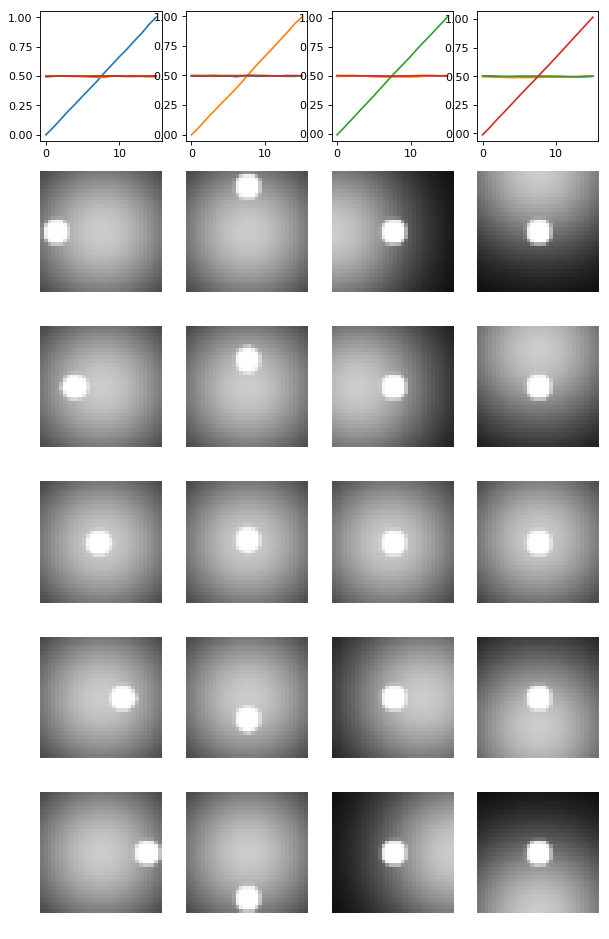
\includegraphics[width=3.375in]{entangle_analysis_supervised_anddata.png}
     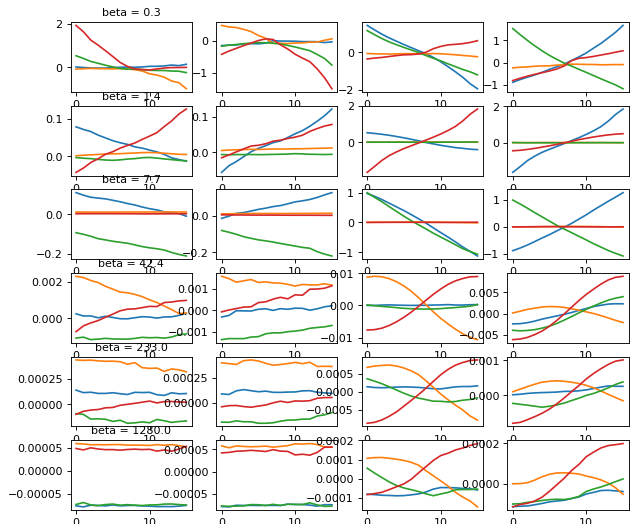
\includegraphics[width=3.375in]{entangle_analysis_betaVAE.png}
  % \end{center}
  \caption{\textbf{Circles dataset and varying levels of entangled representations. [PLACEHOLDER!]}}{(middle, but will be top) The circles dataset, with one generating factor changing in each column (from left to right: circle horizontal and vertical locations, Gaussian horizontal and vertical locations). (top, but will be middle) A perfectly disentangled representation. As one generative factor linearly increases, one unique latent variable also linearly increases while the rest are constant. (bottom) In entangled representations, as one generative factor changes, multiple latent factors change.}
  \label{fig:dataset}
\end{figure}

We first assessed the level of disentanglement existing models can achieve in extremely simple settings, without dynamics,  where perfect disentanglement should be achievable. We constructed a simple dataset in which each image (32x32 pixels) contains a white circle which is drawn over an isotropic Gaussian (see figure~\ref{fig:dataset}a). We randomly varied the positions of each objects while keeping size and intensity fixed. Therefore, there are 4 generative factors for this dataset: the horizontal and vertical position of each object. An ideal encoder for these images that is perfectly disentangled is one with four latent variables, where each one uniquely maps to one of the four generative factors (see figure~\ref{fig:dataset}b). An entangled representation would be one in which multiple latent variables change when varying a single generative factor, and potentially nonlinearly (see figure~\ref{fig:dataset}c).

As a basic control, we wanted to verify that a perfectly disentangled encoder could be achieved by training a simple encoder network with supervision to map its four latent variables directly to the generative factors. The encoder network has four convolutional layers, each with a stride of 2, and a rectified linear (ReLU) output nonlinearity. It is followed by a fully connected layer that maps to the four latent factors. Figure~\ref{fig:dataset}b indeed shows the results from this experiment, demonstrating that this architecture is capable of representing the underlying generative factors in a disentangled way.

Next, we trained \bvae with the same encoder network architecture and a decoder network with the size-matched fully connected and deconvolutional layers in reverse, for different $\beta$ values. The resulting representations are entangled (figure~\ref{fig:dataset}c), and become less informative for higher $\beta$ values.

\begin{figure}[t!]
  % \begin{center}
     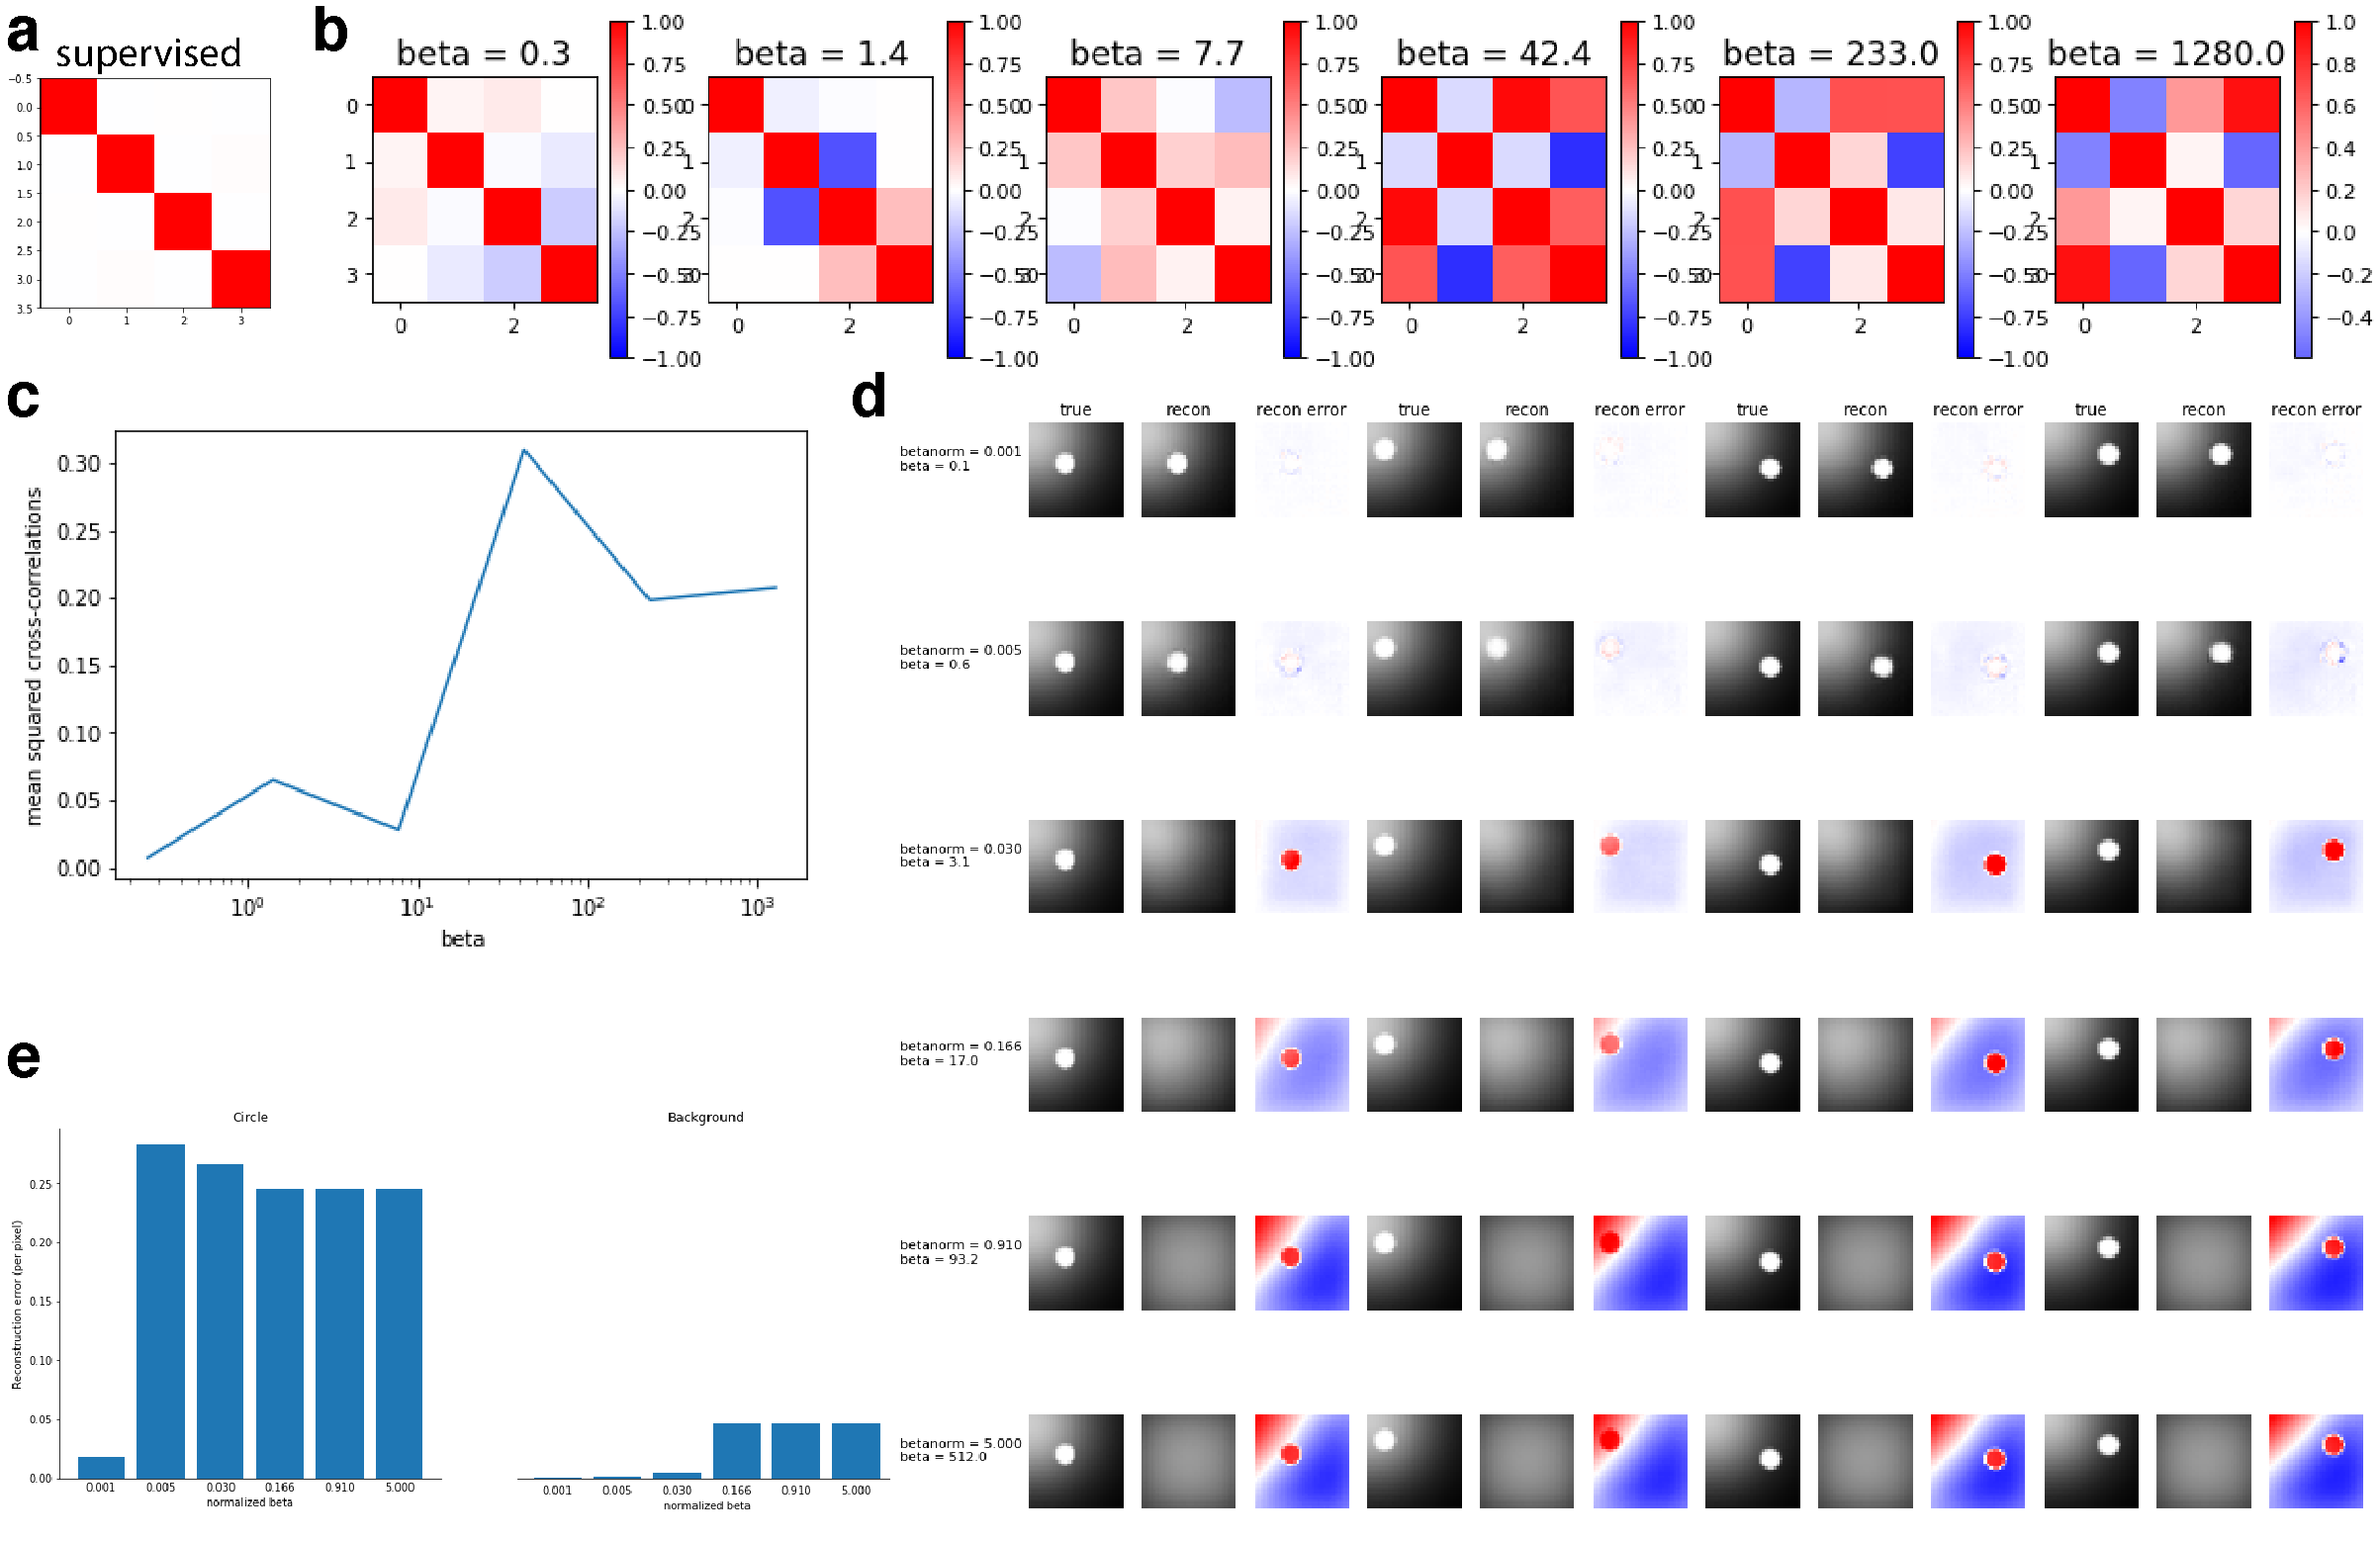
\includegraphics[width=3.375in]{analyses.pdf}
  % \end{center}
  \caption{\textbf{\bvae latent correlation analyses and reconstructions. [PLACEHOLDER!]}}{(a) Supervised encoder latent variable correlations in response to the experiments depicted in figure~\ref{fig:dataset}a show no covariation: they are perfectly disentangled. (b) The same plot as (a), but for \bvae with different $\beta$ values. (c) The mean of the squared off-diagonal entries in the correlation matrices shown in (b). Covariation of latent variables increases with increasing $\beta$, indicating increasing entanglement. (d) For each column containing three images, the left most is the true input image, the middle is the \bvae reconstruction, and on the right is the difference between the two. Note that the circle objects disappear from the reconstructions for all but the lowest two $\beta$ values. (e) Reconstruction error per pixel, as a function of $\beta$, computed either on pixels inside the circle (left) or outside (right).}
  \label{fig:analyses}
\end{figure}

Another way to assess entanglement is to ask how correlated each latent variable is with the other latent variables (figure~\ref{fig:analyses}(a-b)). The representation learned through supervised training shows no correlations between latents. For increasing $\beta$, \bvae latents showed increasing correlations with each other (figure~\ref{fig:analyses}(b-c)). Reconstructions from the \bvae models, however, were good for the lowest two $\beta$s tested, but systematically failed for higher $\beta$ (figure~\ref{fig:analyses}d). Specifically, with increasing $\beta$, first, the white circle completely disappeared but the Gaussian was still reproduced reasonably well. Further increasing $\beta$, the Gaussian was also replaced by a similar shape that is always centered, consistent with the notion that the network has reached its ``auto-decoding'' limit, where the latents are completely ignored \cite{Alemi2017}. This was further quantified with the observation that reconstruction loss on our circles and Gaussians dataset, considered on a per-pixel basis, reaches higher levels for the circle than for the background at lower $\beta$s (figure~\ref{fig:analyses}e).
% In order to assess the effects of adding dynamics into models of disentanglement, we created a dynamic version of the dataset that comprised linear motion of the foreground circle.  ...


\section{Conclusion}

With these simulations, we hope to lay the foundation for using DNN methods for unsupervised and semi-supervised learning to probe how disentangled representations of objects could emerge. We first sought to understand how well existing approaches to disentanglement could perform on a simple task in which perfect disentanglement is possible. Further, we wanted to apply this approach to multiple ``objects'' (in this case, a circle and a Gaussian) are present, rather than their focus on characteristics of a single object or category. We found the popular \bvae architecture to come close to full disentanglement on our dataset of circles and Gaussians, but never quite reach it. Its level of disentanglement and reconstruction quality further declined with increasing $\beta$. This is somewhat at odds with previous predictions, in which one should trade-off with the other \cite{Higgins2017,Alemi2017}, but is likely due to our choice of a low number of latent variables.

We hypothesize that a further inductive bias is necessary to produce truly disentangled representations. Objects are not static; they exist in a continuous world. The putative generative factors that determine an object’s appearance are likely to remain stable (e.g., the object's identity) or vary smoothly and slowly over time (e.g., the object's position or rotation) \cite{Wiskott2002}. This inductive bias could support feature learning in biological systems.

We propose that a representation which factorizes static properties and their dynamics will lead to better disentanglement. Previous approaches using dynamics as inductive biases for unsupervised learning settings combined VAEs with recurrent neural networks and Kalman filters \cite{Krishnan2015}, probabilistic graphical models \cite{Karl2016,Johnson2016}, and linear dynamical systems \cite{Archer2016,Johnson2016,Watter2015,Fraccaro2017a}. The latter study specifically used linear dynamics to learn more disentangled representations. In order to assess the effects of adding dynamics into models of disentanglement, we created a dynamic version of the dataset with linear, translational motion of the foreground circle, and will test our models on it.

\bigskip

%\section{Acknowledgments}
%Place acknowledgments (including funding information) in a section at
%the end of the paper.

\bibliographystyle{apacite}
\setlength{\bibleftmargin}{.125in}
\setlength{\bibindent}{-\bibleftmargin}
\bibliography{refs}

\end{document}
